% 第三章：复积分与柯西理论

\chapter{复积分与柯西理论}

\begin{wulibj}[本章导读]
第二章里，我们已经知道：解析函数不是普通的``二维函数''，它满足柯西--黎曼条件，和调和函数、二维势场、局部保角性都有紧密联系。接下来，一个非常自然的问题就是：如果我们把这样的函数沿复平面中的曲线积分，会发生什么？

一开始，复积分看上去只是把实变积分里的 $\mathrm{d}x$ 换成了 $\mathrm{d}z$。但真正学下去以后，你会发现差别远不止于此。对于一般连续函数，积分当然会依赖路径；可对于解析函数，情况会突然变得异常整齐：闭路积分往往为零，积分可能只由端点决定，甚至区域内部一点的函数值都能由边界上的积分表示出来。

本章要完成下面几件事：
\begin{enumerate}
    \item 建立复积分的定义、参数化计算方法和基本性质；
    \item 理解路径无关、原函数与闭路积分之间的关系；
    \item 掌握柯西积分定理\index{柯西积分定理}与柯西积分公式这两条主线定理；
    \item 为下一章的泰勒展开、解析函数刚性以及第五章的留数理论作准备。
\end{enumerate}

如果把本章压缩成一条主线，那就是
\[
    \begin{aligned}
        \text{解析函数}
        &\Longrightarrow \text{闭路积分为零}
        \Longrightarrow \text{路径无关与原函数} \\
        &\Longrightarrow \text{柯西积分公式}
        \Longrightarrow \text{解析函数的刚性}.
    \end{aligned}
\]
请大家带着这个主线往下看。这样后面遇到各种公式时，就不容易把它们看成彼此孤立的技巧。
\end{wulibj}

% ========== 第一节 ==========
\section{复积分的定义、参数化与基本性质}

\subsection{复积分的定义}

\begin{dingliyi}{复积分}{}
设 $C$ 是复平面上一条有向光滑曲线，起点为 $A$，终点为 $B$。函数 $f(z)$ 在 $C$ 上有定义。将 $C$ 任意分割成 $n$ 段，分点为 $z_0 = A, z_1, \ldots, z_n = B$。在每个小弧段上任意取点 $\zeta_k$，作和
\begin{equation}
    S_n = \sum_{k=1}^{n} f(\zeta_k)(z_k - z_{k-1}) = \sum_{k=1}^{n} f(\zeta_k)\Delta z_k
\end{equation}
若当 $\max|\Delta z_k| \to 0$ 时，$S_n$ 的极限存在且与分割方式和 $\zeta_k$ 的取法无关，则称此极限为 $f(z)$ 沿曲线 $C$ 的\textbf{复积分}，记作
\begin{equation}
    \int_C f(z)\,\mathrm{d}z = \lim_{\max|\Delta z_k| \to 0} \sum_{k=1}^{n} f(\zeta_k)\Delta z_k
\end{equation}
\end{dingliyi}

\begin{figure}[htbp]
\centering
\begin{tikzpicture}[scale=1.2]
    % 曲线 C
    \draw[blue, thick, domain=0:90] plot ({2*cos(\x)}, {2*sin(\x)});
    \node[blue] at (2.3, 1) {$C$};
    
    % 分割点
    \foreach \angle/\label in {0/A, 30/z_1, 60/z_2, 90/B} {
        \fill[red] ({2*cos(\angle)}, {2*sin(\angle)}) circle (2pt);
        \node[below right] at ({2*cos(\angle)}, {2*sin(\angle)}) {$\label$};
    }
    
    % 中间点
    \fill[green!60!black] ({2*cos(15)}, {2*sin(15)}) circle (1.5pt);
    \node[above] at ({2*cos(15)}, {2*sin(15)}) {$\zeta_1$};
    
    % 坐标轴
    \draw[->, gray] (-0.5, 0) -- (3, 0) node[right] {$x$};
    \draw[->, gray] (0, -0.5) -- (0, 3) node[above] {$y$};
\end{tikzpicture}
\caption{复积分的定义：曲线分割}
\label{fig:complex-int-def}
\end{figure}

\subsection{复积分的参数化与计算}

设 $f(z) = u(x, y) + \mathrm{i}v(x, y)$，$z = x + \mathrm{i}y$，$\mathrm{d}z = \mathrm{d}x + \mathrm{i}\mathrm{d}y$。则
\begin{align}
    \int_C f(z)\,\mathrm{d}z &= \int_C (u + \mathrm{i}v)(\mathrm{d}x + \mathrm{i}\mathrm{d}y) \\
    &= \int_C (u\,\mathrm{d}x - v\,\mathrm{d}y) + \mathrm{i}\int_C (v\,\mathrm{d}x + u\,\mathrm{d}y)
\end{align}

这把复积分化为两个实线积分。

\begin{lizi}{}{}
计算 $\displaystyle\int_C z\,\mathrm{d}z$，其中 $C$ 是从 $0$ 到 $1 + \mathrm{i}$ 的直线段。

\begin{jie}
    参数化曲线：$z(t) = t(1 + \mathrm{i})$，$t \in [0, 1]$。
    
    则 $\mathrm{d}z = (1 + \mathrm{i})\,\mathrm{d}t$，$z = t(1 + \mathrm{i})$。
    
    \begin{align}
        \int_C z\,\mathrm{d}z &= \int_0^1 t(1 + \mathrm{i}) \cdot (1 + \mathrm{i})\,\mathrm{d}t \\
        &= (1 + \mathrm{i})^2 \int_0^1 t\,\mathrm{d}t \\
        &= 2\mathrm{i} \cdot \frac{1}{2} = \mathrm{i}
    \end{align}
\end{jie}
\end{lizi}

\subsection{复积分的基本性质}

\begin{dingli}{复积分的基本性质}{}
设 $f(z)$ 和 $g(z)$ 沿曲线 $C$ 可积，则：
\begin{enumerate}
    \item $\displaystyle\int_C [f(z) + g(z)]\,\mathrm{d}z = \int_C f(z)\,\mathrm{d}z + \int_C g(z)\,\mathrm{d}z$
    \item $\displaystyle\int_C kf(z)\,\mathrm{d}z = k\int_C f(z)\,\mathrm{d}z$（$k$ 为常数）
    \item $\displaystyle\int_{C_1 + C_2} f(z)\,\mathrm{d}z = \int_{C_1} f(z)\,\mathrm{d}z + \int_{C_2} f(z)\,\mathrm{d}z$
    \item $\displaystyle\int_{C^-} f(z)\,\mathrm{d}z = -\int_C f(z)\,\mathrm{d}z$（$C^-$ 是 $C$ 的反向曲线）
    \item $\displaystyle\left|\int_C f(z)\,\mathrm{d}z\right| \leq \int_C |f(z)|\,|\mathrm{d}z| = \int_C |f(z)|\,\mathrm{d}s$
\end{enumerate}
\end{dingli}

\begin{zhu}{}{}
性质5称为\textbf{积分估值不等式}，其中 $\mathrm{d}s$ 是弧长微元。它给出积分模的上界。
\end{zhu}

% ========== 第二节 ==========
\section{路径无关、原函数与复积分基本公式}

\begin{wulibj}[为什么这里先谈路径无关]
上一节我们已经看到，复积分的定义本身是沿曲线作和，因此对一般函数来说，积分自然会依赖路径。可一旦某个函数存在原函数，积分就会突然变得和实变积分很像：它只和起点、终点有关，而与中间具体怎样走无关。

这一节先把这种``如果有原函数，就会路径无关''的思路讲清楚。下一节再用柯西积分定理说明：为什么在单连通区域里，解析函数恰好会拥有这种特殊性质。
\end{wulibj}

\subsection{什么叫积分与路径无关}

设 $z_1,z_2$ 是区域 $D$ 内两点，$C_1,C_2$ 是连接 $z_1$ 与 $z_2$ 的两条分段光滑曲线。若对任意这样的两条曲线都有
\[
    \int_{C_1} f(z)\,\mathrm{d}z = \int_{C_2} f(z)\,\mathrm{d}z,
\]
则称 $f(z)$ 在区域 $D$ 内的积分\textbf{与路径无关}。

\begin{zhu}{}{}
``与路径无关''不是一个定义性的空话，而是一个很强的性质。它的意思是：从同一点出发走到同一点终止时，中间绕不绕弯、沿哪条路走，都不会改变积分值。
\end{zhu}

\subsection{原函数与复积分的基本公式}

\begin{dingliyi}{原函数}{}
设 $f(z)$ 在区域 $D$ 内连续。若存在 $F(z)$ 使得
\[
    F'(z)=f(z)
\]
在 $D$ 内成立，则称 $F(z)$ 是 $f(z)$ 的一个\textbf{原函数}。
\end{dingliyi}

\begin{dingli}{有原函数时的复积分基本公式}{}
\index{牛顿@牛顿（Newton）}\index{莱布尼茨@莱布尼茨（Leibniz）}
设 $f(z)$ 在区域 $D$ 内有原函数 $F(z)$。若 $C$ 是 $D$ 内一条从 $z_1$ 到 $z_2$ 的分段光滑曲线，则
\[
    \int_C f(z)\,\mathrm{d}z = F(z_2)-F(z_1).
\]
\end{dingli}

\begin{proof}
沿曲线 $C$ 作参数化
\[
    z=z(t),\qquad a\le t\le b,
\]
其中
\[
    z(a)=z_1,\qquad z(b)=z_2.
\]
于是
\[
    \int_C f(z)\,\mathrm{d}z
    = \int_a^b f(z(t))z'(t)\,\mathrm{d}t
    = \int_a^b F'(z(t))z'(t)\,\mathrm{d}t.
\]
由链式法则，
\[
    \frac{\mathrm{d}}{\mathrm{d}t}F(z(t)) = F'(z(t))z'(t),
\]
因此
\[
    \int_C f(z)\,\mathrm{d}z
    = \int_a^b \frac{\mathrm{d}}{\mathrm{d}t}F(z(t))\,\mathrm{d}t
    = F(z(b))-F(z(a))
    = F(z_2)-F(z_1).
\]
这就得到了所需公式。
\end{proof}

\begin{tuilun}{有原函数时积分与路径无关}{}
若 $f(z)$ 在区域 $D$ 内有原函数，则它在 $D$ 内的积分与路径无关；特别地，对任意闭曲线 $C$，都有
\[
    \oint_C f(z)\,\mathrm{d}z = 0.
\]
\end{tuilun}

\begin{proof}
若 $C_1,C_2$ 都从 $z_1$ 走到 $z_2$，则由上一定理，
\[
    \int_{C_1} f(z)\,\mathrm{d}z = F(z_2)-F(z_1)=\int_{C_2} f(z)\,\mathrm{d}z.
\]
所以积分与路径无关。

当 $C$ 是闭曲线时，起点与终点重合，于是
\[
    \oint_C f(z)\,\mathrm{d}z = F(z_1)-F(z_1)=0.
\]
\end{proof}

\begin{tishi}[这一节和下一节的关系]
到目前为止，我们只是说明了：\textbf{如果}原函数存在，那么积分就会路径无关。下一节真正关键的内容是：为什么单连通区域里的解析函数会满足闭路积分为零，从而反过来获得原函数。这正是柯西积分定理\index{柯西积分定理}的威力所在。
\end{tishi}

% ========== 第三节 ==========
\section{柯西积分定理与闭路积分\index{柯西积分定理}}

\subsection{定理的陈述}

设 $f(z)$ 在\keyword{单连通区域} $D$ 内解析，$C$ 是 $D$ 内任意一条简单闭曲线，则
\begin{dingli}{柯西积分定理}{}
设 $f(z)$ 在单连通区域 $D$ 内解析，$C$ 是 $D$ 内任意一条简单闭曲线，则
\[
    \oint_C f(z)\,\mathrm{d}z = 0
\]
\end{dingli}

\begin{figure}[htbp]
\centering
\begin{tikzpicture}[scale=1.2]
    % 区域 D
    \draw[fill=blue!10, thick] plot[smooth cycle] coordinates {(0,0) (2,0) (3,1) (2.5,2.5) (1,2.5) (-0.5,1.5)};
    \node at (1.2, 1.3) {$D$};
    
    % 闭曲线 C
    \draw[red, thick, ->] (1, 0.5) to[out=60, in=180] (2, 1.5) to[out=0, in=90] (2.5, 0.8) to[out=-90, in=0] (1.5, 0.3) to[out=180, in=-60] cycle;
    \node[red] at (2.2, 2) {$C$};
    
    \node at (1.2, -0.5) {单连通区域内};
\end{tikzpicture}
\caption{柯西积分定理\index{柯西积分定理}：单连通区域内的闭路积分为零}
\label{fig:cauchy-thm}
\end{figure}

\subsection{定理的证明（格林公式方法）}

\begin{proof}
设 $f(z) = u + \mathrm{i}v$，则
\begin{equation}
    \oint_C f(z)\,\mathrm{d}z = \oint_C (u\,\mathrm{d}x - v\,\mathrm{d}y) + \mathrm{i}\oint_C (v\,\mathrm{d}x + u\,\mathrm{d}y)
\end{equation}

由格林公式：
\begin{align}
    \oint_C (u\,\mathrm{d}x - v\,\mathrm{d}y) &= \iint_D \left(-\frac{\partial v}{\partial x} - \frac{\partial u}{\partial y}\right)\mathrm{d}x\mathrm{d}y \\
    \oint_C (v\,\mathrm{d}x + u\,\mathrm{d}y) &= \iint_D \left(\frac{\partial u}{\partial x} - \frac{\partial v}{\partial y}\right)\mathrm{d}x\mathrm{d}y
\end{align}

由 C-R 条件：$u_x = v_y$，$u_y = -v_x$。因此两个积分的被积函数都为零，故
\begin{equation}
    \oint_C f(z)\,\mathrm{d}z = 0
\end{equation}
\end{proof}

\begin{zhu}{}{}
这个证明要求 $u_x, u_y, v_x, v_y$ 连续。更一般的证明（不要求偏导数连续）需要更细致的分析。
\end{zhu}

\subsection{闭路积分为零带来的后果}

\begin{dingli}{单连通区域中原函数的存在性}{}
若 $f(z)$ 在单连通区域 $D$ 内解析，则 $f(z)$ 在 $D$ 内存在原函数。
\end{dingli}

\begin{proof}
取定一点 $z_0\in D$。对任意 $z\in D$，定义
\[
    F(z)=\int_{z_0}^{z} f(\zeta)\,\mathrm{d}\zeta,
\]
其中积分路径取在区域 $D$ 内。

由柯西积分定理\index{柯西积分定理}，任意闭曲线上的积分都为零，因此两点之间的积分与路径无关，所以 $F(z)$ 的定义是良好的。

再仿照上一节的参数化讨论，可以证明
\[
    F'(z)=f(z).
\]
因此 $F(z)$ 正是 $f(z)$ 的一个原函数。
\end{proof}

\begin{tishi}[三件事其实连在一起]
到这里为止，我们已经看到了下面这条主线：
\[
    \text{闭路积分为零} \Longrightarrow \text{路径无关} \Longrightarrow \text{原函数存在}.
\]
而在单连通区域里，解析函数之所以拥有这些性质，根源正是柯西积分定理。换句话说，复积分之所以``突然变整齐''，并不是偶然，而是解析性带来的结果。
\end{tishi}

% ========== 第四节 ==========
\section{多连通区域与典型闭路积分}

\begin{wulibj}[为什么单连通条件不能随手丢掉]
上一节的柯西积分定理是在单连通区域里成立的。很多同学第一次看到这个条件时，会把它当成一句技术性限制；但一进入多连通区域，情形就会立刻改变。最典型的例子就是
\[
    \frac{1}{z-z_0}.
\]
它除了 $z_0$ 以外处处解析，可一旦曲线把 $z_0$ 围住，闭路积分就不再是零。

这一节的任务，就是让大家真正看见：区域里的``洞''会怎样改变积分行为。
\end{wulibj}

\subsection{多连通区域的柯西积分定理\index{柯西积分定理}}

\begin{dingli}{多连通区域的柯西积分定理}{}
设 $f(z)$ 在多连通区域 $D$ 内解析，$C$ 是 $D$ 内的简单闭曲线，$C_1, C_2, \ldots, C_n$ 是被 $C$ 包围的内部边界。若这些曲线都取正向（外边界逆时针，内边界顺时针），则
\begin{equation}
    \oint_C f(z)\,\mathrm{d}z = \sum_{k=1}^{n} \oint_{C_k} f(z)\,\mathrm{d}z
\end{equation}
\end{dingli}

\begin{figure}[htbp]
\centering
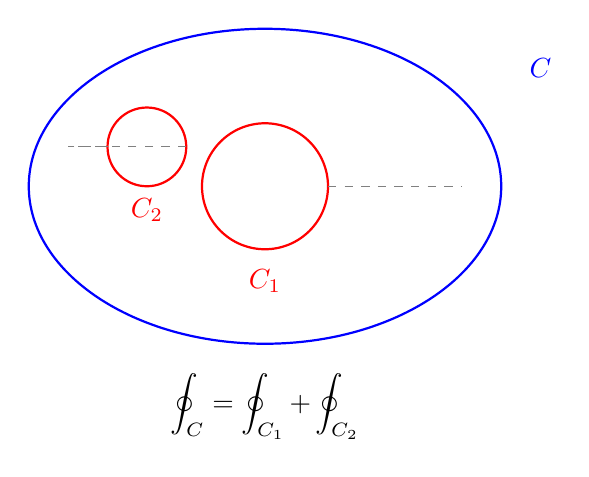
\begin{tikzpicture}[scale=1.0]
    % 外边界
    \draw[blue, thick, ->] (0,0) ellipse (3 and 2);
    \node[blue] at (3.5, 1.5) {$C$};
    
    % 内边界
    \draw[red, thick, <-] (0, 0) circle (0.8);
    \node[red] at (0, -1.2) {$C_1$};
    
    \draw[red, thick, <-] (-1.5, 0.5) circle (0.5);
    \node[red] at (-1.5, -0.3) {$C_2$};
    
    % 割线
    \draw[gray, dashed] (0.8, 0) -- (2.5, 0);
    \draw[gray, dashed] (-1, 0.5) -- (-2.5, 0.5);
    \draw[gray, dashed] (-2, 0.5) -- (-2.5, 0.5);
    
    \node at (0, -2.8) {$\displaystyle\oint_C = \oint_{C_1} + \oint_{C_2}$};
\end{tikzpicture}
\caption{多连通区域：外边界积分等于内边界积分之和}
\label{fig:multi-connected}
\end{figure}

\begin{lizi}{}{}
计算 $\displaystyle\oint_C \frac{1}{z - z_0}\,\mathrm{d}z$，其中 $C$ 是包围 $z_0$ 的简单闭曲线。

\begin{jie}
    以 $z_0$ 为圆心、$r$ 为半径作小圆 $C_r$，取逆时针方向。
    
    由多连通区域的柯西积分定理\index{柯西积分定理}：
    \begin{equation}
        \oint_C \frac{1}{z - z_0}\,\mathrm{d}z = \oint_{C_r} \frac{1}{z - z_0}\,\mathrm{d}z
    \end{equation}
    
    在 $C_r$ 上，$z - z_0 = r\mathrm{e}^{\mathrm{i}\theta}$，$\mathrm{d}z = r\mathrm{i}\mathrm{e}^{\mathrm{i}\theta}\,\mathrm{d}\theta$：
    \begin{equation}
        \oint_{C_r} \frac{1}{z - z_0}\,\mathrm{d}z = \int_0^{2\pi} \frac{r\mathrm{i}\mathrm{e}^{\mathrm{i}\theta}}{r\mathrm{e}^{\mathrm{i}\theta}}\,\mathrm{d}\theta = \int_0^{2\pi} \mathrm{i}\,\mathrm{d}\theta = 2\pi\mathrm{i}
    \end{equation}
\end{jie}
\end{lizi}

\begin{tishi}[重要结论]
这个例子的结果非常重要：$\displaystyle\oint_C \frac{1}{z - z_0}\,\mathrm{d}z = 2\pi\mathrm{i}$（$z_0$ 在 $C$ 内部）。这是导出柯西积分公式的基础。
\end{tishi}

% ========== 第三节 ==========
\section{柯西积分公式}

\subsection{公式的推导}

\begin{dingli}{柯西积分公式}{}
设 $f(z)$ 在简单闭曲线 $C$ 所围区域 $D$ 内解析，在 $\bar{D} = D \cup C$ 上连续，$z_0$ 是 $D$ 内任意一点，则
\[
    f(z_0) = \frac{1}{2\pi\mathrm{i}}\oint_C \frac{f(z)}{z - z_0}\,\mathrm{d}z
\]
\end{dingli}

\begin{proof}
考虑积分 $\displaystyle\oint_C \frac{f(z)}{z - z_0}\,\mathrm{d}z$。

以 $z_0$ 为圆心、$r$ 为半径作小圆 $C_r$。由多连通区域的柯西积分定理\index{柯西积分定理}：
\begin{equation}
    \oint_C \frac{f(z)}{z - z_0}\,\mathrm{d}z = \oint_{C_r} \frac{f(z)}{z - z_0}\,\mathrm{d}z
\end{equation}

注意到 $f(z) = f(z_0) + [f(z) - f(z_0)]$，所以
\begin{equation}
    \oint_{C_r} \frac{f(z)}{z - z_0}\,\mathrm{d}z = f(z_0)\oint_{C_r} \frac{1}{z - z_0}\,\mathrm{d}z + \oint_{C_r} \frac{f(z) - f(z_0)}{z - z_0}\,\mathrm{d}z
\end{equation}

第一项等于 $f(z_0) \cdot 2\pi\mathrm{i}$。

对于第二项，由于 $f(z)$ 连续，对于任意 $\varepsilon > 0$，存在 $\delta > 0$，当 $|z - z_0| < \delta$ 时，$|f(z) - f(z_0)| < \varepsilon$。

取 $r < \delta$，则
\begin{equation}
    \left|\oint_{C_r} \frac{f(z) - f(z_0)}{z - z_0}\,\mathrm{d}z\right| \leq \frac{\varepsilon}{r} \cdot 2\pi r = 2\pi\varepsilon
\end{equation}

由 $\varepsilon$ 的任意性，第二项为零。因此
\begin{equation}
    \oint_C \frac{f(z)}{z - z_0}\,\mathrm{d}z = 2\pi\mathrm{i} f(z_0)
\end{equation}
\end{proof}

\begin{wulibj}[物理意义：平均值性质]
柯西积分公式表明：解析函数\index{解析函数}在一点的值等于它在该点周围边界上的``平均值''（加权积分）。这说明解析函数\index{解析函数}的值由边界值完全确定，体现了解析函数\index{解析函数}的``刚性''。
\end{wulibj}

\begin{tishi}[深入理解：解析函数的``刚性'']
柯西积分公式揭示了解析函数\index{解析函数}的一个惊人性质——让我们来仔细品味一下。

公式告诉我们：只要知道了解析函数\index{解析函数} $f(z)$ 在边界 $C$ 上的值，就能唯一确定它在整个区域内部的值！

这和实变函数完全不同。对于实函数 $y = f(x)$，知道 $f(0) = 1$，你无法确定 $f(0.5)$ 是多少——可能有无数种函数通过 $(0, 1)$ 这个点。但解析函数\index{解析函数}不同：知道了边界上的值，内部就完全确定了。

这就是所谓的``刚性''：解析函数\index{解析函数}就像一块刚性的板，你不能随意弯曲它——一旦固定了边界，整块板就固定了。

更进一步，高阶导数公式告诉我们：解析函数\index{解析函数}在某点的各阶导数也都由边界值决定！这意味着：
\begin{enumerate}
    \item 解析函数\index{解析函数}在一点知道它的值，就知道了它所有导数的值，从而知道了它在整个邻域内的值（泰勒展开）。
    \item 解析函数\index{解析函数}不可能只在某个小区域为零——如果它在一段弧上为零，就必须在整个区域内为零。
    \item 解析函数\index{解析函数}不可能有``局部极值''——最大模原理说 $|f(z)|$ 的最大值只能在边界上达到。
\end{enumerate}

这些性质都源于一个核心：解析函数\index{解析函数}是一个高度``约束''的对象，它的各个部分紧密联系，牵一发而动全身。
\end{tishi}

\subsection{柯西积分公式的应用}

\begin{lizi}{}{}
计算 $\displaystyle\oint_C \frac{\mathrm{e}^z}{z - 1}\,\mathrm{d}z$，其中 $C$ 是 $|z| = 2$（逆时针方向）。

\begin{jie}
    $f(z) = \mathrm{e}^z$ 在 $C$ 内解析，$z_0 = 1$ 在 $C$ 内。
    
    由柯西积分公式：
    \begin{equation}
        \oint_C \frac{\mathrm{e}^z}{z - 1}\,\mathrm{d}z = 2\pi\mathrm{i} f(1) = 2\pi\mathrm{i} \cdot \mathrm{e}
    \end{equation}
\end{jie}
\end{lizi}

% ========== 第六节 ==========
\section{柯西积分公式的直接推论}

\subsection{高阶导数公式}

\begin{dingli}{高阶导数公式}{}
在柯西积分公式的条件下，$f(z)$ 在 $D$ 内有\keyword{任意阶导数}，且
\[
    f^{(n)}(z_0) = \frac{n!}{2\pi\mathrm{i}}\oint_C \frac{f(z)}{(z - z_0)^{n+1}}\,\mathrm{d}z
\]
\end{dingli}

\begin{proof}
对柯西积分公式两边对 $z_0$ 求导。形式地，
\begin{align}
    f'(z_0) &= \frac{1}{2\pi\mathrm{i}}\oint_C \frac{f(z)}{(z - z_0)^2}\,\mathrm{d}z \\
    f''(z_0) &= \frac{2}{2\pi\mathrm{i}}\oint_C \frac{f(z)}{(z - z_0)^3}\,\mathrm{d}z
\end{align}
一般地，归纳可得结论。严格证明需要验证积分号下求导的合法性。
\end{proof}

\begin{tishi}[惊人结论]
解析函数\index{解析函数}有任意阶导数！这是与实变函数的根本区别。一个实函数可以一阶可导但二阶不可导，但复变函数一旦可导就无穷次可导。
\end{tishi}

\begin{lizi}{}{}
计算 $\displaystyle\oint_C \frac{\sin z}{(z - \mathrm{i})^3}\,\mathrm{d}z$，其中 $C$ 是 $|z| = 2$。

\begin{jie}
    $f(z) = \sin z$，$z_0 = \mathrm{i}$，$n = 2$。
    
    由高阶导数公式：
    \begin{equation}
        \oint_C \frac{\sin z}{(z - \mathrm{i})^3}\,\mathrm{d}z = \frac{2\pi\mathrm{i}}{2!} f''(\mathrm{i})
    \end{equation}
    
    $f''(z) = -\sin z$，所以 $f''(\mathrm{i}) = -\sin(\mathrm{i}) = -\mathrm{i}\sinh(1)$。
    
    因此
    \begin{equation}
        \oint_C \frac{\sin z}{(z - \mathrm{i})^3}\,\mathrm{d}z = \pi\mathrm{i} \cdot (-\mathrm{i}\sinh(1)) = \pi\sinh(1)
    \end{equation}
\end{jie}
\end{lizi}

% ========== 第七节 ==========
\section{解析性的积分判据：莫雷拉定理（选读）}

\begin{wulibj}[为什么把莫雷拉定理放在章末]
到前一节为止，本章主线其实已经完整了：复积分的定义、柯西积分定理\index{柯西积分定理}、多连通区域中的典型闭路积分、柯西积分公式以及高阶导数公式，这些内容已经足以支撑下一章的泰勒展开。

莫雷拉\index{莫雷拉@莫雷拉（Morera）}（Morera）定理回答的是一个反方向的问题：如果我们只知道某个连续函数对任意闭曲线的积分都为零，能不能反过来推出它解析？这个问题很漂亮，也很重要，但它更像是对本章主线的一次回看，因此放在章末作为选读更合适。
\end{wulibj}

\subsection{莫雷拉定理}

\begin{dingli}{莫雷拉定理}{}
设 $f(z)$ 在区域 $D$ 内连续，且对于 $D$ 内任意简单闭曲线 $C$，有 $\oint_C f(z)\,\mathrm{d}z = 0$，则 $f(z)$ 在 $D$ 内解析。
\end{dingli}

\begin{proof}
由条件，积分 $\int_{z_0}^z f(\zeta)\,\mathrm{d}\zeta$ 与路径无关。定义
\begin{equation}
    F(z) = \int_{z_0}^z f(\zeta)\,\mathrm{d}\zeta
\end{equation}
类似于柯西积分定理\index{柯西积分定理}证明的逆过程，可以证明 $F'(z) = f(z)$。

因此 $f(z)$ 是 $F(z)$ 的导数。由于解析函数\index{解析函数}的导数仍解析（高阶导数公式的推论），$f(z)$ 在 $D$ 内解析。
\end{proof}

\begin{tishi}[柯西积分定理的逆定理]
    莫雷拉\index{莫雷拉@莫雷拉（Morera）}（Morera）定理是柯西积分定理\index{柯西积分定理}的逆定理。两者结合，我们得到：
\begin{equation}
    f \text{ 解析} \quad \Longleftrightarrow \quad \oint_C f(z)\,\mathrm{d}z = 0 \text{（对任意闭曲线）}
\end{equation}
\end{tishi}

\begin{tishi}[和下一章的衔接]
刘维尔定理和最大模原理虽然同样从柯西积分公式长出来，但它们更适合和泰勒展开、解析函数刚性放在一起系统讨论。因此它们将放到下一章``解析函数的整体性质与刚性''中出现。这样安排以后，本章主线会更集中，下一章的逻辑也会更顺。
\end{tishi}

% ========== 本章小结 ==========
\section{本章小结}

\subsection{核心定理}

\begin{enumerate}
    \item \textbf{有原函数时的复积分基本公式}：$\displaystyle \int_C f(z)\,\mathrm{d}z = F(z_2)-F(z_1)$
    \item \textbf{柯西积分定理\index{柯西积分定理}}：单连通区域内解析函数\index{解析函数}沿闭曲线积分等于零
    \item \textbf{单连通区域中的原函数存在性}：解析函数在单连通区域内存在原函数
    \item \textbf{柯西积分公式}：$\displaystyle f(z_0) = \frac{1}{2\pi\mathrm{i}}\oint_C \frac{f(z)}{z - z_0}\,\mathrm{d}z$
    \item \textbf{高阶导数公式}：$\displaystyle f^{(n)}(z_0) = \frac{n!}{2\pi\mathrm{i}}\oint_C \frac{f(z)}{(z - z_0)^{n+1}}\,\mathrm{d}z$
    \item \textbf{莫雷拉定理（选读）}：闭路积分为零可反推函数解析
\end{enumerate}

\subsection{重要结论}

\begin{itemize}
    \item 在单连通区域里，解析函数\index{解析函数}的积分与路径无关，并且存在原函数
    \item 典型闭路积分 $\displaystyle\oint_C \frac{1}{z-z_0}\,\mathrm{d}z = 2\pi\mathrm{i}$ 是柯西积分公式的基础
    \item 解析函数\index{解析函数}在一点的值和各阶导数都可以由边界积分表示
    \item 下一章的泰勒展开、刘维尔定理和最大模原理，都将从本章结果继续生长出来
\end{itemize}

% ========== 习题 ==========
\section{习题}

\textbf{基础题}

\begin{enumerate}
    \item 计算下列积分：
    \begin{enumerate}
        \item $\displaystyle\int_C z^2\,\mathrm{d}z$，$C$ 是从 $0$ 到 $1 + \mathrm{i}$ 的直线段
        \item 分别沿两条路径计算 $\displaystyle\int_C \overline{z}\,\mathrm{d}z$：一路径为从 $0$ 到 $1+\mathrm{i}$ 的直线段，另一路径先沿实轴从 $0$ 到 $1$，再沿竖直线段从 $1$ 到 $1+\mathrm{i}$
    \end{enumerate}
    
    \item 利用柯西积分公式计算：
    \begin{enumerate}
        \item $\displaystyle\oint_C \frac{\cos z}{z - \pi}\,\mathrm{d}z$，$C$ 是 $|z| = 4$
        \item $\displaystyle\oint_C \frac{\mathrm{e}^z}{z^2}\,\mathrm{d}z$，$C$ 是 $|z| = 1$
    \end{enumerate}
\end{enumerate}

\textbf{综合题}

\begin{enumerate}[resume]
    \item 设 $f(z)$ 在区域 $D$ 内有原函数 $F(z)$。证明：$f(z)$ 在 $D$ 内的积分与路径无关，并说明为什么任意闭曲线上的积分都为零。
    
    \item 计算 $\displaystyle\oint_C \frac{z}{(z - 1)(z - 2)}\,\mathrm{d}z$，其中 $C$ 分别为：
    \begin{enumerate}
        \item $|z| = 1.5$
        \item $|z| = 3$
    \end{enumerate}
    
    \item 说明为什么 $\displaystyle \frac{1}{z}$ 在穿孔平面 $\mathbb{C}\setminus\{0\}$ 上不可能有单值原函数。
\end{enumerate}

\textbf{挑战题}

\begin{enumerate}[resume]
    \item 用参数化方法直接证明：若 $C$ 是圆周 $|z-z_0|=r$ 的逆时针方向，则
    \[
        \oint_C \frac{1}{z-z_0}\,\mathrm{d}z = 2\pi\mathrm{i}.
    \]
    
    \item 设 $f(z)$ 在区域 $D$ 内连续，且对 $D$ 内任意闭曲线 $C$ 都有
    \[
        \oint_C f(z)\,\mathrm{d}z = 0.
    \]
    取定 $z_0\in D$，定义
    \[
        F(z)=\int_{z_0}^{z} f(\zeta)\,\mathrm{d}\zeta.
    \]
    试证明 $F'(z)=f(z)$，并说明这与莫雷拉定理有什么关系。
\end{enumerate}
